\chapter{原子与分子}\label{ch:g7:atoms-and-molecules}

取一滴水，把它切成两半。每一半仍是水。把其中一半
再切成两半，再切，再切。你能一直切下去吗，还是
会得到一小块东西，再切一次便
不再是水？公元前 400 年左右，希腊
思想家德谟克利特猜出了答案：物质由一些细小的、无法切开的颗粒构成，
他称之为\emph{原子}，取自希腊语，
意为“不可切割”。此后又经过两千多年，
十九世纪化学家的工作，才把这一猜想变为
科学。本章介绍这些粒子——原子——以及它们
如何组成分子。

\begin{recall}
纯净物，如水或氧气，由一种化学物种构成；
混合物，如空气，则含有多种化学物种
（\cref{ch:g6:pure-substances-and-mixtures}）。空气约五分之四是
氮，五分之一是氧（\cref{ch:g4:air-a-mixture-of-gases}）。
\end{recall}

\section{原子}

\begin{definition}[原子]\label{def:g7:atoms-and-molecules:atom}
一切物质都由极其微小的粒子构成，这些粒子称为
\emph{原子}\index{原子}。自然界中仅有约一百种不同的
原子，而每种物质——水、空气、铁、
糖、我们自己的身体——都由其中的几种原子构成。
\end{definition}

\begin{proposition}[原子很小]\label{prop:g7:atoms-and-molecules:tiny}
% ledger: const:a0, earth:diameter (8 cm apple: 12756 km / 8 cm = 1.6 x 10^8;
% 0.1-0.15 nm x 1.6 x 10^8 = 1.7-2.4 cm, a small cherry)
最小的原子是氢原子，直径约为一毫米的
千万分之一；其他原子至多大几倍。一千万
个氢原子排成一行，长度正好是一毫米。
想象一下：若把一只苹果吹大到地球那么大，它的每个
原子大约只有一颗小樱桃那么大。
\end{proposition}

\begin{remark}[看不见却看得见]\label{rem:g7:atoms-and-molecules:seen}
用光做照明的显微镜都无法看到原子：原子远小于
光波。自 1980 年代起，一种特殊的显微镜用极细的针尖
探测物体表面，制作出的图像中，单个
原子呈现为一个个小凸起。
\end{remark}

\begin{definition}[原子符号]\label{def:g7:atoms-and-molecules:symbol}
每种原子都有名称和\emph{符号}\index{符号}：
由一个大写字母构成，有时后接一个小写字母。
同一符号在各种语言中都一样。
\end{definition}

\begin{center}
\small
\begin{tabular}{llll|llll}
\hline
原子 & 符号 & & 模型颜色 & 原子 & 符号 & & 模型颜色 \\
\hline
氢 & \ce{H} & \tikz\node[aH]{}; & 白色 & 钠 & \ce{Na} & \tikz\node[aNa]{}; & 紫色 \\
碳 & \ce{C} & \tikz\node[aC]{}; & 黑色 & 硫 & \ce{S} & \tikz\node[aS]{}; & 黄色 \\
氮 & \ce{N} & \tikz\node[aN]{}; & 蓝色 & 氯 & \ce{Cl} & \tikz\node[aCl]{}; & 绿色 \\
氧 & \ce{O} & \tikz\node[aO]{}; & 红色 & 铁、铜 & \ce{Fe}, \ce{Cu} & &——\\
\hline
\end{tabular}
\end{center}

\begin{remark}[符号的来历]\label{rem:g7:atoms-and-molecules:latin}
多数符号取自元素名称的首字母：\ce{H} 代表氢，
\ce{C} 代表碳，\ce{O} 代表氧。少数符号来自较古老的拉丁文
名称：\ce{Na} 代表钠（\emph{natrium}），\ce{Fe} 代表铁
（\emph{ferrum}），\ce{Cu} 代表铜（\emph{cuprum}）。第二个字母
总是小写：\ce{Co} 是钴原子，而带大写 O 的 CO
则完全是另一回事。
\end{remark}

\begin{history}[道尔顿的原子，1808 年]
1808 年，化学家约翰·道尔顿发表了一张当时已知原子的表，
每种原子都画成一个带有自身符号的小圆圈。他是
第一个指出同种原子的质量都相同，并
认为化学家可以比较这些质量。但他还推测水是
一个氢原子与一个氧原子结合而成；又过了五十年
化学家才达成共识：一个水分子含有\emph{两个}
氢原子。
\end{history}

\begin{omfigure}
\begin{minipage}[b]{0.3\linewidth}\centering
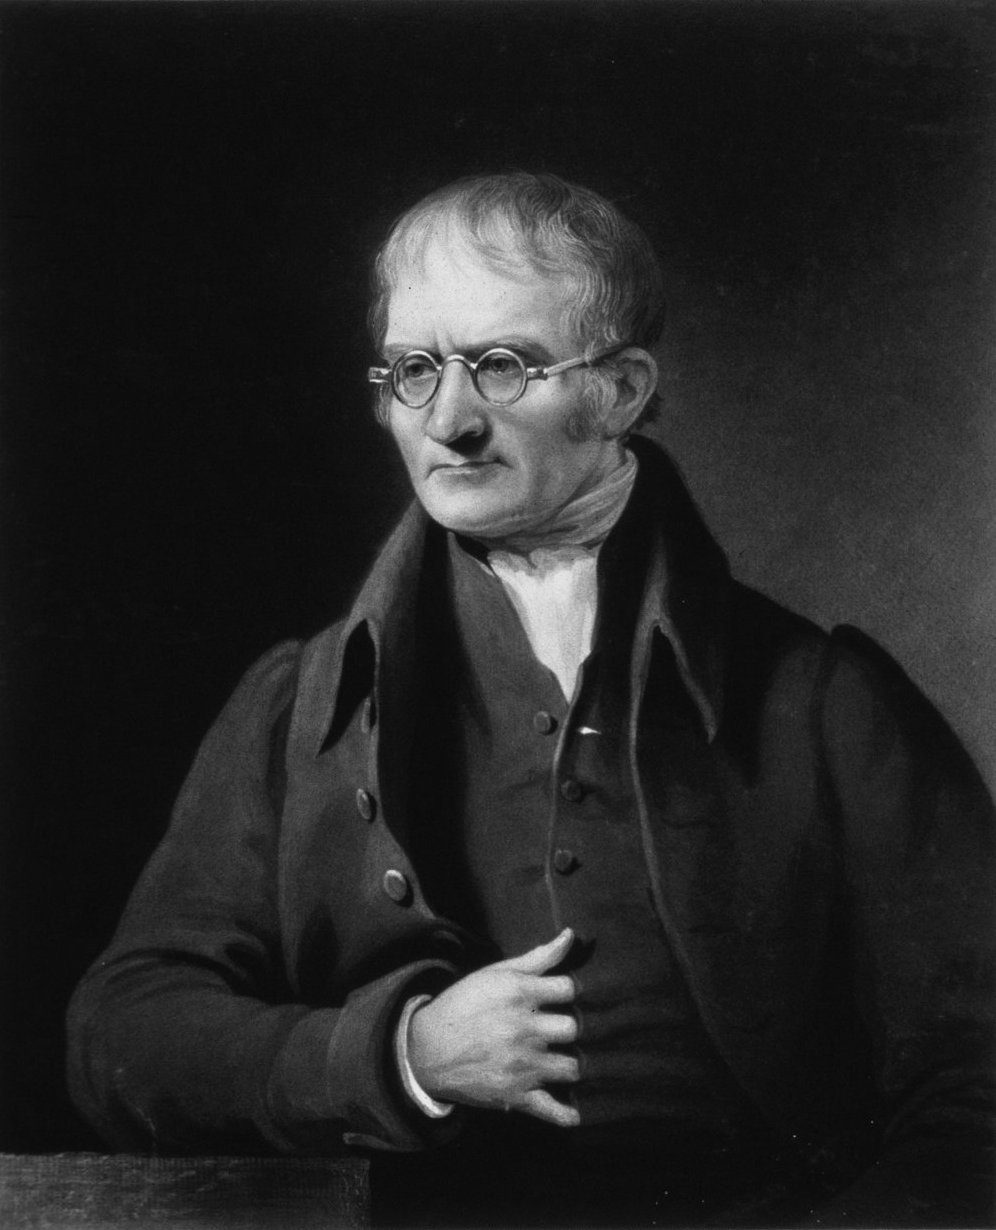
\includegraphics[width=\linewidth]{images/book1/dalton.jpg}

{\small 约翰·道尔顿（1766--1844）。}
\end{minipage}\hfill
\begin{minipage}[b]{0.66\linewidth}\centering
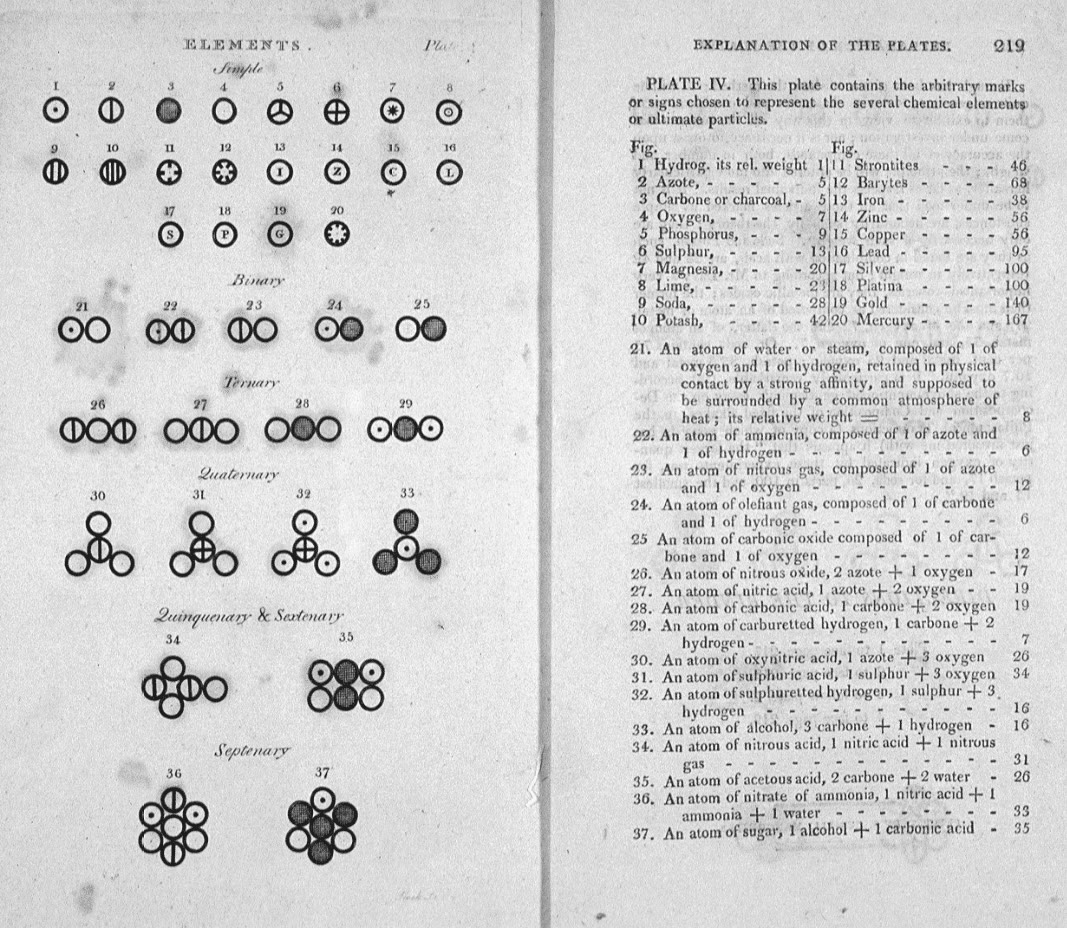
\includegraphics[width=\linewidth]{images/book1/dalton-symbols.jpg}

{\small 道尔顿 1808 年的表：他的水，符号 21，是
一个氢的圆圈与一个氧的圆圈并排。}
\end{minipage}
\end{omfigure}

\section{分子}

\begin{definition}[分子]\label{def:g7:atoms-and-molecules:molecule}
\emph{分子}\index{分子}是紧密结合在一起的一组原子。
分子是仍保持该物质性质的最小粒子；
仍属该物质：水分子是能够存在的最小一份
水。
\end{definition}

\begin{example}[七种分子]\label{ex:g7:atoms-and-molecules:seven}
\begin{itemize}
  \item \emph{氢}分子：两个氢原子；
  \item 呼吸所需的\emph{氧}分子：两个氧原子；
  \item 占空气五分之四的\emph{氮}分子：两个
        氮原子；
  \item \emph{水}分子：两个氢原子和一个氧
        原子；
  \item 呼出的\emph{二氧化碳}分子：一个
        碳原子和两个氧原子；
  \item \emph{甲烷}分子，是天然气的主要成分，
        在燃气灶中燃烧：一个碳原子和四个氢原子；
  \item \emph{一氧化二氮}分子，一种麻醉气体：两个
        氮原子和一个氧原子。
\end{itemize}
\end{example}

\begin{omfigure}
\begin{tikzpicture}[font=\small]
  % hydrogen
  \begin{scope}[xshift=0cm]
    \node[aH] (a) at (-0.25,0) {}; \node[aH] (b) at (0.25,0) {};
    \begin{scope}[on background layer]\draw[bond] (a.center) -- (b.center);\end{scope}
    \node at (0,-1.05) {氢};
  \end{scope}
  % oxygen
  \begin{scope}[xshift=2.6cm]
    \node[aO] (a) at (-0.33,0) {}; \node[aO] (b) at (0.33,0) {};
    \begin{scope}[on background layer]
      \draw[bond, line width=1.1pt] ([yshift=1.6pt]a.center) -- ([yshift=1.6pt]b.center);
      \draw[bond, line width=1.1pt] ([yshift=-1.6pt]a.center) -- ([yshift=-1.6pt]b.center);
    \end{scope}
    \node at (0,-1.05) {氧};
  \end{scope}
  % nitrogen
  \begin{scope}[xshift=5.2cm]
    \node[aN] (a) at (-0.33,0) {}; \node[aN] (b) at (0.33,0) {};
    \begin{scope}[on background layer]
      \foreach \d in {-2.4,0,2.4}
        \draw[bond, line width=0.9pt] ([yshift=\d pt]a.center) -- ([yshift=\d pt]b.center);
    \end{scope}
    \node at (0,-1.05) {氮};
  \end{scope}
  % water
  \begin{scope}[xshift=7.8cm, yshift=0.2cm]
    \node[aO] (o) at (0,0) {};
    \node[aH] (h1) at (-0.62,-0.48) {}; \node[aH] (h2) at (0.62,-0.48) {};
    \begin{scope}[on background layer]
      \draw[bond] (o.center) -- (h1.center); \draw[bond] (o.center) -- (h2.center);
    \end{scope}
    \node at (0,-1.25) {水};
  \end{scope}
  % carbon dioxide
  \begin{scope}[xshift=0.9cm, yshift=-2.7cm]
    \node[aO] (a) at (-0.85,0) {}; \node[aC] (c) at (0,0) {}; \node[aO] (b) at (0.85,0) {};
    \begin{scope}[on background layer]
      \foreach \d in {-1.6,1.6} {
        \draw[bond, line width=1.1pt] ([yshift=\d pt]a.center) -- ([yshift=\d pt]c.center);
        \draw[bond, line width=1.1pt] ([yshift=\d pt]c.center) -- ([yshift=\d pt]b.center);}
    \end{scope}
    \node at (0,-1.05) {二氧化碳};
  \end{scope}
  % methane
  \begin{scope}[xshift=4.4cm, yshift=-2.6cm]
    \node[aC] (c) at (0,0) {};
    \node[aH] (h1) at (0,0.78) {};
    \node[aH] (h2) at (-0.74,-0.3) {};
    \node[aH] (h3) at (0.74,-0.3) {};
    \begin{scope}[on background layer]
      \draw[bond] (c.center) -- (h1.center); \draw[bond] (c.center) -- (h2.center);
      \draw[bond] (c.center) -- (h3.center);
    \end{scope}
    \draw[bond] (c.center) -- (0.22,-0.52);
    \node[aH] at (0.24,-0.58) {};
    \node at (0,-1.15) {甲烷};
  \end{scope}
  % nitrous oxide
  \begin{scope}[xshift=7.8cm, yshift=-2.7cm]
    \node[aN] (a) at (-0.8,0) {}; \node[aN] (b) at (0,0) {}; \node[aO] (c) at (0.8,0) {};
    \begin{scope}[on background layer]
      \foreach \d in {-1.6,1.6} {
        \draw[bond, line width=1.1pt] ([yshift=\d pt]a.center) -- ([yshift=\d pt]b.center);
        \draw[bond, line width=1.1pt] ([yshift=\d pt]b.center) -- ([yshift=\d pt]c.center);}
    \end{scope}
    \node at (0,-1.05) {一氧化二氮};
  \end{scope}
\end{tikzpicture}

{\small 球棍模型展示了
\cref{ex:g7:atoms-and-molecules:seven}中的七种分子。每根短棍代表两个原子之间的
一个化学键；有些原子之间共用两根或三根短棍，
其原因留待后面的章节解释。}
\end{omfigure}

\begin{proposition}[纯净物与混合物中的分子]\label{prop:g7:atoms-and-molecules:pure}
由分子构成的纯净物中，所有分子都相同：
纯水中只含水分子。混合物中含有
几种不同的分子：空气主要是氮分子和
氧分子，氮分子数约为氧分子数的四倍，另有少量
以单个原子形式存在的氩原子，以及极少量的二氧化碳分子。
\end{proposition}

\begin{omfigure}
\begin{tikzpicture}[font=\small,
    sN/.style={aN, minimum size=3.0mm}, sO/.style={aO, minimum size=2.9mm},
    sH/.style={aH, minimum size=2.1mm}, sAr/.style={om atom, ball color=cyan!60, minimum size=3.4mm}]
  % air
  \draw[omGlass, line width=0.6pt] (0,0) rectangle (3.4,3.4);
  \foreach \x/\y/\r in {0.5/0.6/20, 1.6/0.4/-30, 2.8/0.7/75, 0.6/1.7/110,
                        2.0/1.5/10, 2.9/2.0/-60, 0.9/2.8/40, 2.1/2.9/-15}
    \node[sN] at ($(\x,\y)+(\r:0.12)$) {} node[sN] at ($(\x,\y)+(\r+180:0.12)$) {};
  \foreach \x/\y/\r in {1.3/1.1/60, 1.6/2.3/-40}
    \node[sO] at ($(\x,\y)+(\r:0.12)$) {} node[sO] at ($(\x,\y)+(\r+180:0.12)$) {};
  \node[sAr] at (2.9,3.0) {};
  \node[anchor=north] at (1.7,-0.1) {\textbf{空气}：混合物};
  % water
  \begin{scope}[xshift=5.2cm]
    \draw[omGlass, line width=0.6pt] (0,0) rectangle (3.4,3.4);
    \foreach \x in {0,1,2,3,4} \foreach \y in {0,1,2,3,4} {
      \pgfmathsetmacro{\ang}{mod(73*\x+41*\y,360)}
      \begin{scope}[shift={({0.36+0.67*\x},{0.4+0.66*\y})}, rotate=\ang]
        \node[sH] at (-0.16,-0.12) {}; \node[sH] at (0.16,-0.12) {};
        \node[sO] at (0,0) {};
      \end{scope}}
    \node[anchor=north] at (1.7,-0.1) {\textbf{水}：纯净物};
  \end{scope}
\end{tikzpicture}

{\small 极度放大后观察。左图：空气中，氮气分子
（蓝色）远多于氧气分子（红色），而一个氩原子（浅蓝色）独自运动；
气体分子之间相距很远。右图：液态水中，
分子都相同，且彼此接触。}
\end{omfigure}

\section{化学式}

\begin{definition}[化学式]\label{def:g7:atoms-and-molecules:formula}
分子的\emph{化学式}\index{化学式}列出其
原子的符号，每个符号后面跟一个写在右下方的小数字，
即\emph{下标}\index{下标}，表示该种原子在分子中含有的个数。
下标为 1 时不写出。
\end{definition}

\begin{example}[七种化学式]\label{ex:g7:atoms-and-molecules:formulas}
\cref{ex:g7:atoms-and-molecules:seven}中各分子的
化学式如下：
\begin{center}
\begin{tabular}{lcl}
\hline
分子 & 化学式 & 原子 \\
\hline
氢气 & \ce{H2} & 2 个氢原子 \\
氧气 & \ce{O2} & 2 个氧原子 \\
氮气 & \ce{N2} & 2 个氮原子 \\
水 & \ce{H2O} & 2 个氢原子、1 个氧原子 \\
二氧化碳 & \ce{CO2} & 1 个碳原子、2 个氧原子 \\
甲烷 & \ce{CH4} & 1 个碳原子、4 个氢原子 \\
一氧化二氮 & \ce{N2O} & 2 个氮原子、1 个氧原子 \\
\hline
\end{tabular}
\end{center}
\end{example}

\begin{method}[读化学式]\label{met:g7:atoms-and-molecules:read}
读取分子化学式的方法：
\begin{enumerate}
  \item 将化学式拆分为元素符号，每个符号以大写字母开头；
  \item 读出每个符号后面的下标（没有下标则为 1）；
  \item 将所有下标相加，得到原子总数。
\end{enumerate}
以 \ce{C2H6O}（乙醇，即饮料中的酒精）为例：2 个碳原子、6 个氢原子、
1 个氧原子，共 9 个原子。
\end{method}

\begin{remark}[前面的数字]\label{rem:g7:atoms-and-molecules:coefficient}
写在化学式前面的数字表示分子的个数：\ce{3H2O} 表示
3 个水分子，共含 6 个氢原子和 3 个氧
原子。不要把 \ce{O2}（一个由两个氧原子构成的分子）与
\ce{2O}（两个未结合在一起的氧原子）混淆。
\end{remark}

\begin{example}[厨房中的甲烷]\label{ex:g7:atoms-and-molecules:methane}
燃气灶所用的天然气主要是甲烷 \ce{CH4}。其中每
个分子都由一个碳原子和周围的四个氢原子构成。这种气体
看不见，本身也没有气味：人们闻到的“燃气”气味，
是人为加入的一种物质，以便及时发现漏气。
\end{example}

\begin{omfigure}
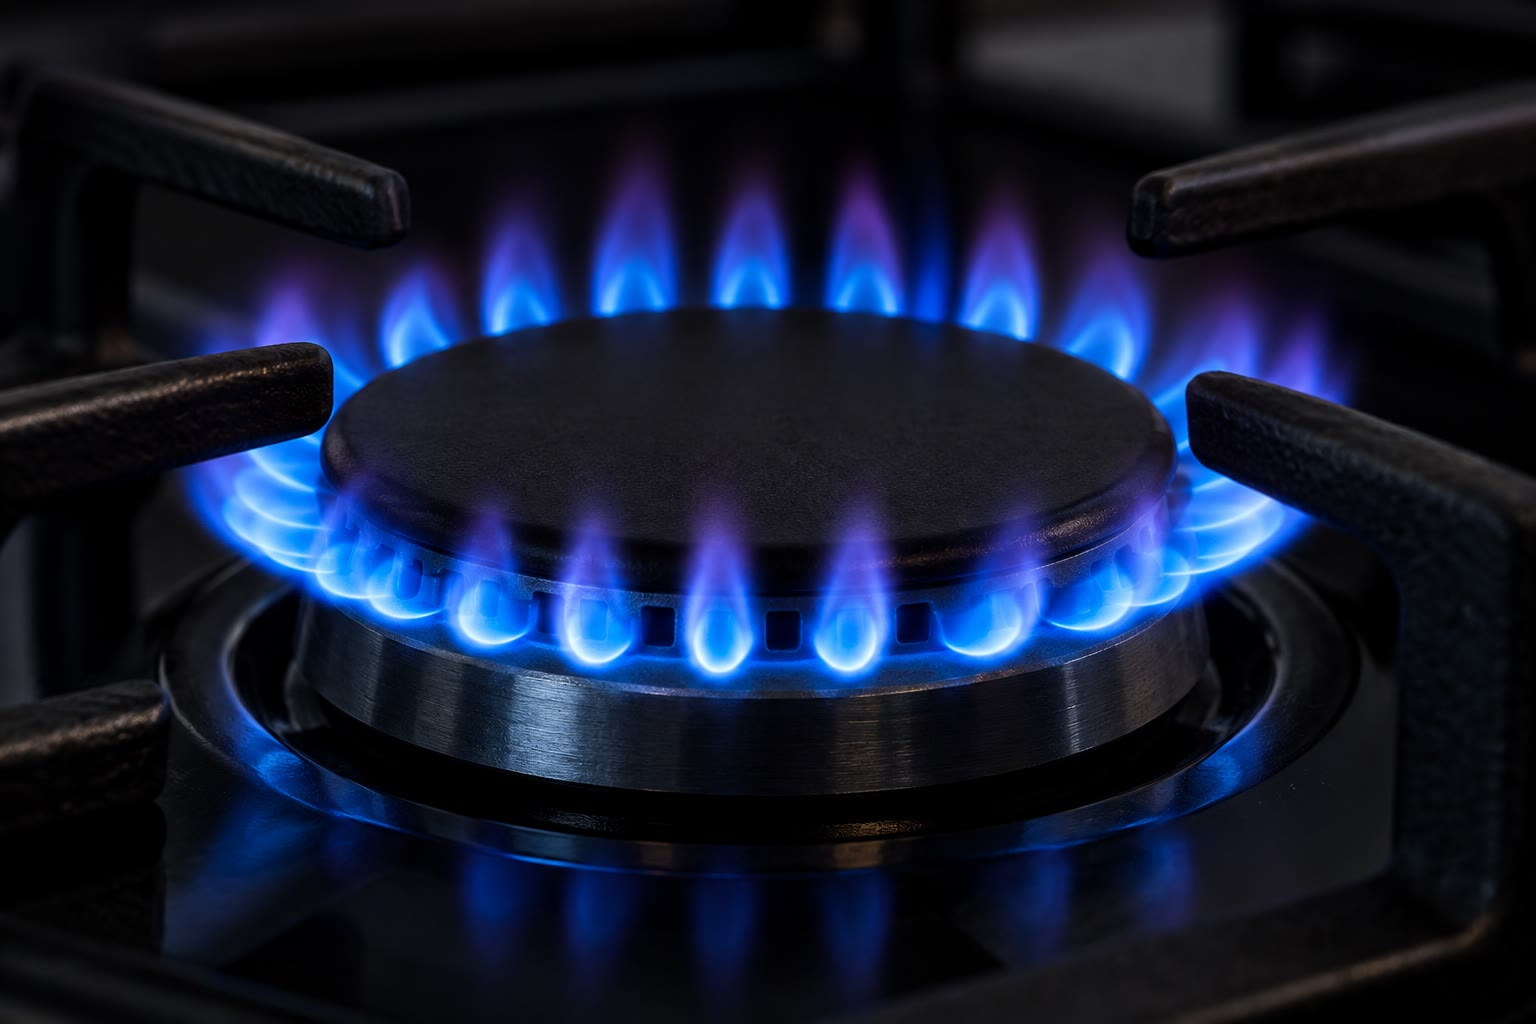
\includegraphics[width=0.5\linewidth]{images/book1/ai/g7-gas-flame.jpg}

{\small 燃气灶的蓝色火焰：天然气中的甲烷正在燃烧。}
\end{omfigure}

\section{分子模型}

\begin{remark}[模型及其颜色]\label{rem:g7:atoms-and-molecules:models}
化学家用\emph{分子模型}表示分子：
小球代表原子，小棍代表原子之间的化学键。颜色是世界各地通用的约定——
碳为黑色、氢为白色、氧为红色、氮为蓝色——
并不是原子的真实颜色，单个原子根本没有颜色。
模型还能显示分子的形状，这是化学式做不到的：
水分子是弯曲的，
二氧化碳分子是直线形的。
\end{remark}

\begin{omfigure}
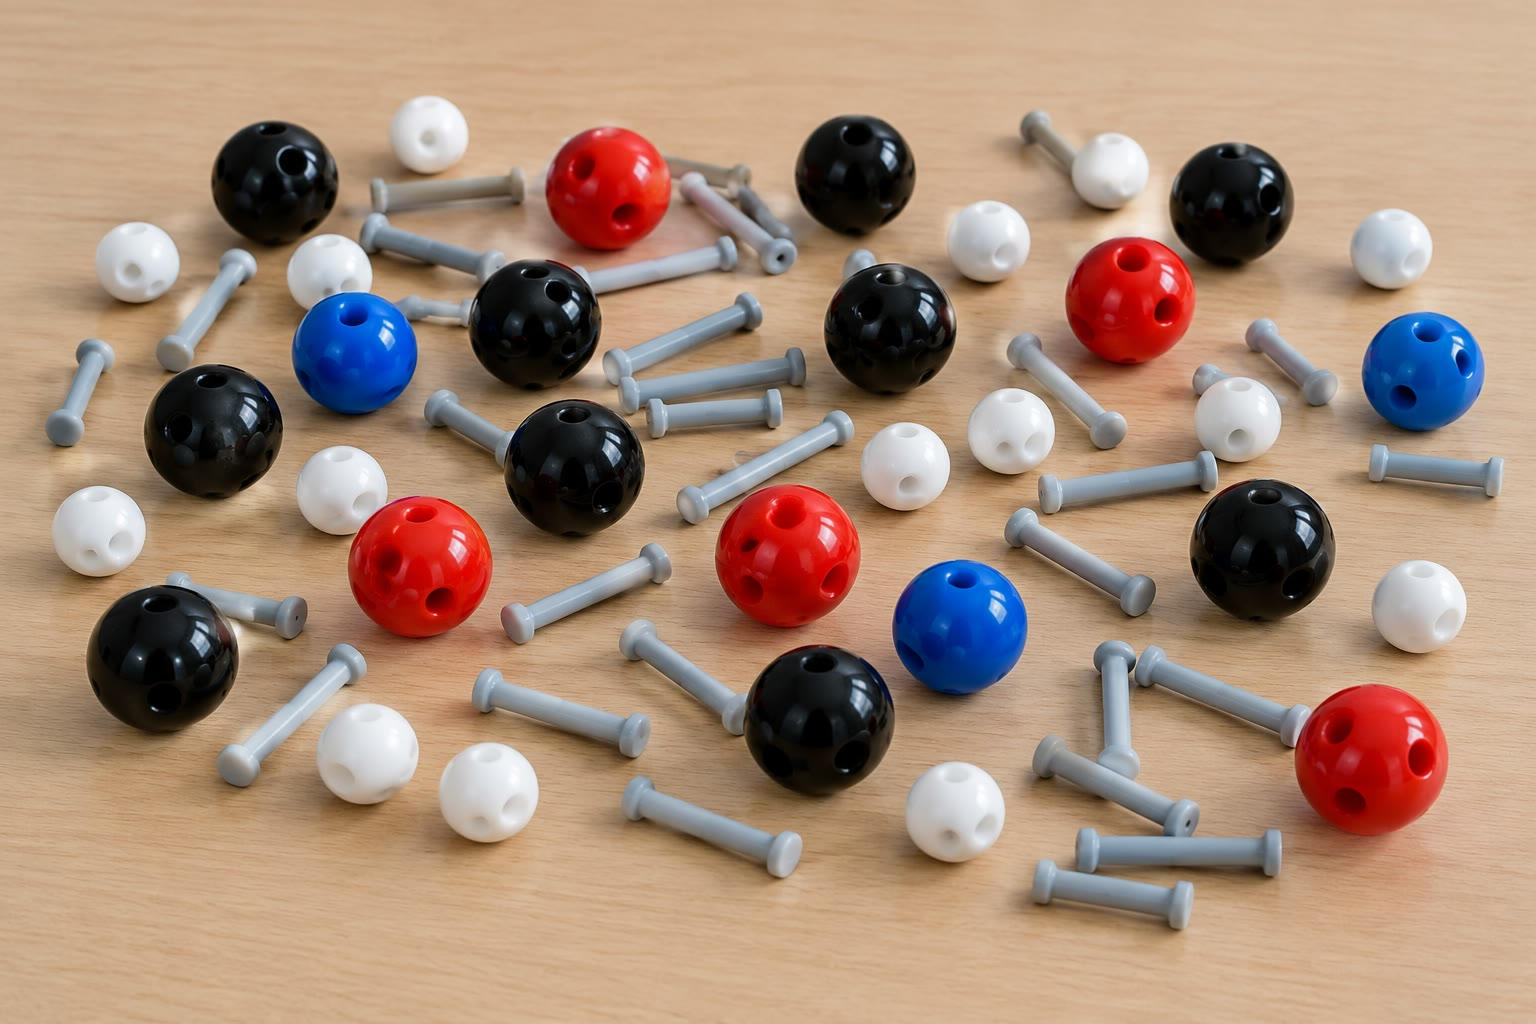
\includegraphics[width=0.5\linewidth]{images/book1/ai/g7-model-kit.jpg}

{\small 分子模型套件：小球代表原子，球上的孔用于插入
代表化学键的小棍。}
\end{omfigure}

\begin{method}[从模型到化学式]\label{met:g7:atoms-and-molecules:model}
由分子模型写出分子化学式的方法：
\begin{enumerate}
  \item 根据颜色判断原子种类；
  \item 数出每种颜色小球的个数；
  \item 写出各元素符号并把个数作为下标，先写碳，
        再写氢，
        其余原子按元素符号字母顺序排列。
\end{enumerate}
一个黑色小球与四个白色小球相连：一个碳原子、四个氢原子，
即 \ce{CH4}。
\end{method}

\section{练习}

\begin{exercise}[$\star$]\label{exo:g7:atoms-and-molecules:1}
什么是原子？什么是分子？
\end{exercise}

\begin{exercise}[$\star$]\label{exo:g7:atoms-and-molecules:2}
写出下列元素的符号：氢、碳、氮、氧、钠和
铁。
\end{exercise}

\begin{exercise}[$\star$]\label{exo:g7:atoms-and-molecules:3}
一个二氧化碳分子（\ce{CO2}）中，每种原子各有
多少个？一共有多少个原子？
\end{exercise}

\begin{exercise}[$\star$]\label{exo:g7:atoms-and-molecules:4}
请写出分子 \ce{H2O}、\ce{O2}、\ce{CH4} 和 \ce{N2} 的名称。
\end{exercise}

\begin{exercise}[$\star$]\label{exo:g7:atoms-and-molecules:5}
二氧化氮是一种存在于污染空气中的棕色气体，
其一个分子由 1 个氮原子和 2 个氧原子构成。写出它的化学式。
\end{exercise}

\begin{exercise}[$\star\star$]\label{exo:g7:atoms-and-molecules:6}
说明 \ce{O2} 与 \ce{2O} 的区别，以及 \ce{CO}
与 \ce{Co} 的区别。
\end{exercise}

\begin{exercise}[$\star\star$]\label{exo:g7:atoms-and-molecules:7}
在下列物质中，氢原子与氧原子各有多少个？
\ce{3H2O} 中呢？\ce{5O2} 中呢？
\end{exercise}

\begin{exercise}[$\star\star$]\label{exo:g7:atoms-and-molecules:8}
一个模型由 1 个黑球与 2 个红球连接而成。说出这些
原子的名称，写出化学式，并命名该分子。
\end{exercise}

\begin{exercise}[$\star\star$]\label{exo:g7:atoms-and-molecules:9}
在道尔顿的表中，水由 1 个氢原子和 1 个氧
原子构成。写出道尔顿心目中的化学式，
并说明他的水分子缺少多少个原子。
\end{exercise}

\begin{exercise}[$\star\star$]\label{exo:g7:atoms-and-molecules:10}
纯净水是混合物吗？空气呢？请通过描述每种物质
所含的分子加以回答。
\end{exercise}

\begin{exercise}[$\star\star\star$]\label{exo:g7:atoms-and-molecules:11}
一个氢原子的直径约为一千万分之一毫米。
将氢原子一个挨一个排成一列，要使这条线长 \qty{1}{cm}，
需要多少个氢原子？若这条线长与足球场的长度相当，即 \qty{100}{m}，又需要多少个？
\end{exercise}

\begin{exercise}[$\star\star\star$]\label{exo:g7:atoms-and-molecules:12}
葡萄糖是为我们细胞提供能量的糖，其化学式为
\ce{C6H12O6}。一个葡萄糖分子含有多少个原子？其中
氢原子占百分之几？碳原子占百分之几？
\end{exercise}

\section{问题：一次呼吸中的原子}

\begin{problem}[{周末问题——数一数呼吸的空气中的原子，
比较空气进入肺部前后的情况}]
\label{pb:g7:atoms-and-molecules:1}
% ledger: air:N2, air:O2, air:Ar (78.08 / 20.95 / 0.93 rounded to 78 / 21 / 1),
% breath:O2, breath:CO2, breath:N2 (expired air: 16 / 4 / 78, water vapour removed)
氮气不参与肺部的气体交换，因此可以作为参照。
在干燥空气中，每 78 个氮分子大约对应 21 个氧分子
和 1 个氩原子，共 100 个粒子
（分子或单个原子）。呼出的空气除去水蒸气后，同样的 78 个
氮分子同时伴有约 16 个氧分子、4 个
二氧化碳分子和 1 个氩原子。

\medskip
\noindent\textbf{第一部分——我们吸入的空气。}
\begin{enumerate}
  \item 写出氮气、氧气和二氧化碳分子的化学式，
        并给出每种分子所含的原子数。
  \item 氩以原子计数，而不以分子计数。这说明了
        氩的什么性质？
  \item 在这 100 个吸入的空气粒子中，
        含有多少个氮原子？多少个氧原子？
  \item 这 100 个粒子中共有多少个原子？
  \item 这些原子中，氮原子占百分之几？结果取
        最接近的整数。
\end{enumerate}

\medskip
\noindent\textbf{第二部分——我们呼出的空气。}
\begin{enumerate}[resume]
  \item 在与同样的 78 个氮分子相伴的呼出空气中，
        氧分子中含有多少个氧原子？
        二氧化碳分子中呢？一共多少个？
  \item 与第 3 题对比，缺少了多少个氧原子？这些氧原子
        去了哪种分子中？该分子由体内利用食物中的氢生成，
        并在此随水蒸气排出。
  \item 吸入的空气中含有多少个碳原子？呼出的空气中
        呢？
  \item 空气不会把碳原子带入肺部。呼出气体中的碳原子
        从何而来？（想一想身体用来维持
        生命的是什么。）
  \item 有多少个氧分子消失了，又有多少个二氧化碳
        分子出现了？
\end{enumerate}

\medskip
\noindent\textbf{第三部分——计数。}
\begin{enumerate}[resume]
  \item 描述呼出空气中四种粒子各自的球棍模型，
        并说明各球的颜色，
        （氩用一个淡蓝色的单球表示。）
  \item 呼出的干燥空气中共有多少个原子？
        它比吸入的空气多出多少个原子？请解释这一差异，
        并结合增加的碳原子与缺少的氧原子
        加以说明。
\end{enumerate}
\end{problem}
